% vim: set spell spelllang=en tw=100 et sw=4 sts=4 foldmethod=marker foldmarker={{{,}}} :

\documentclass{beamer}

\usepackage{tikz}
\usepackage{xcolor}
\usepackage{complexity}
\usepackage{hyperref}
\usepackage[vlined]{algorithm2e} % algorithms

\usetikzlibrary{shapes, arrows, shadows, calc, positioning, fit}
\usetikzlibrary{decorations.pathreplacing, decorations.pathmorphing, shapes.misc}
\usetikzlibrary{tikzmark}

\colorlet{screenverylightgrey}{black!2!white}
\colorlet{screengrey}{black!30!white}

\definecolor{uofgblue}{rgb}{0, 0.321569, 0.533333}
\colorlet{uofgblue20}{uofgblue!20!white}
\colorlet{uofgblue40}{uofgblue!40!white}
\colorlet{uofgblue60}{uofgblue!60!white}
\colorlet{uofgblue80}{uofgblue!80!white}

\definecolor{uofgstone}{rgb}{0.498039, 0.454902, 0.403922}

\definecolor{uofgtdarkgreen}{rgb}{0.380392, 0.564706, 0.501961}
\definecolor{uofgtlightgreen}{rgb}{0.615686, 0.788235, 0.729412}
\definecolor{uofgtyellow}{rgb}{0.85098, 0.827451, 0.643137}
\definecolor{uofgtorange}{rgb}{0.784314, 0.694118, 0.545098}

% {{{ theme things
\useoutertheme[footline=authorinstitutetitle]{miniframes}
\useinnertheme{rectangles}

\setbeamerfont{block title}{size={}}
\setbeamercolor*{structure}{fg=uofgblue}
\setbeamercolor*{palette primary}{use=structure,fg=black,bg=white}
\setbeamercolor*{palette secondary}{use=structure,fg=black,bg=uofgblue40}
\setbeamercolor*{palette tertiary}{use=structure,fg=white,bg=uofgblue}
\setbeamercolor*{palette quaternary}{fg=white,bg=black}

\setbeamercolor*{titlelike}{parent=palette primary}

\beamertemplatenavigationsymbolsempty

\tikzset{vertex/.style={draw, circle, inner sep=0pt, minimum size=0.5cm, font=\small\bfseries}}
\tikzset{notvertex/.style={vertex, color=white, text=black}}
\tikzset{plainvertex/.style={vertex}}
\tikzset{selectedvertex/.style={vertex, fill=uofgblue}}
\tikzset{vertexc1/.style={vertex, fill=uofgblue40}}
\tikzset{vertexc2/.style={vertex, fill=uofgblue}}
\tikzset{vertexc3/.style={vertex, fill=uofgtdarkgreen}}
\tikzset{vertexc4/.style={vertex, fill=uofgtorange}}
\tikzset{edge/.style={color=screengrey}}
\tikzset{bedge/.style={ultra thick}}
\tikzset{edgel1/.style={ultra thick, color=uofgblue}}
\tikzset{edgel2/.style={ultra thick, color=uofgblue40}}
\tikzset{edgel3/.style={ultra thick, color=uofgtdarkgreen}}
\tikzset{edgel4/.style={ultra thick, color=uofgtorange}}

\setbeamertemplate{title page}
{
    \vbox{}
    \vspace*{0.5cm}
    \begin{centering}
        {\usebeamerfont{title}\inserttitle\par}
        \vskip0.5cm\par
        \begin{beamercolorbox}[sep=8pt,center]{author}
            \usebeamerfont{author}\insertauthor
        \end{beamercolorbox}
        {\usebeamercolor[fg]{titlegraphic}\inserttitlegraphic\par}
    \end{centering}
    \vfill

    \begin{tikzpicture}[remember picture, overlay]
        \node at (current page.north west) {\begin{tikzpicture}[remember picture, overlay]\fill
        [fill=uofgblue, anchor=north west] (0, 0) rectangle (\paperwidth, -1.5cm);\end{tikzpicture}};
        \node [anchor=north west, shift={(0.2cm,-0.2cm)}] at (current page.north west) {\includegraphics*[keepaspectratio=true,scale=0.5]{UoG_keyline.eps}};
    \end{tikzpicture}
}

% }}}

\title{Russian Doll Search}
\author[Ciaran McCreesh]{\textcolor{uofgblue}{Ciaran McCreesh}}

\begin{document}

{
    \usebackgroundtemplate{\includegraphics*[keepaspectratio=true, height=\paperheight]{background.jpg}}
    \begin{frame}[plain]
        \titlepage
    \end{frame}
}

\begin{frame}{An Old Maximum Clique Algorithm}

    \only<1>{
        \centering
        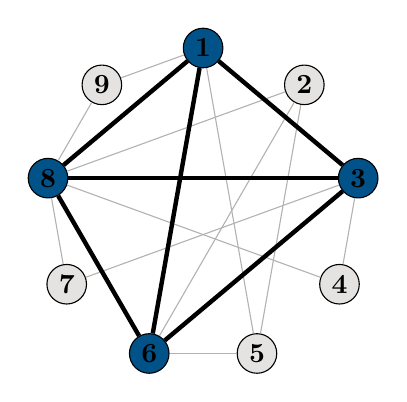
\begin{tikzpicture}%{{{
            \newcount \c
            \foreach \n in {1, ..., 9}{
                \c=\n
                \multiply\c by -40
                \advance\c by 130
                \ifthenelse{\n = 1 \OR \n = 3 \OR \n = 6 \OR \n = 8}{
                    \node[draw, circle, fill=uofgblue, inner sep=2pt] (N\n) at (\the\c:2) {\textbf{\n}};
                }{
                    \node[draw, circle, fill=uofgstone!20!white, inner sep=2pt] (N\n) at (\the\c:2) {\textbf{\n}};
                }
            }

            \draw [edge] (N1) -- (N5); \draw [edge] (N1) -- (N9);
            \draw [edge] (N2) -- (N5); \draw [edge] (N2) -- (N6); \draw [edge] (N2) -- (N8);
            \draw [edge] (N3) -- (N4); \draw [edge] (N3) -- (N7);
            \draw [edge] (N4) -- (N8);
            \draw [edge] (N5) -- (N6);
            \draw [edge] (N7) -- (N8);
            \draw [edge] (N8) -- (N9);

            \draw [bedge] (N1) -- (N3);
            \draw [bedge] (N6) -- (N8);
            \draw [bedge] (N1) -- (N6);
            \draw [bedge] (N1) -- (N8);
            \draw [bedge] (N3) -- (N6);
            \draw [bedge] (N3) -- (N8);
        \end{tikzpicture}%}}}
        \\~
    }

    \only<2>{
        \begin{itemize}
            \item Let $G[V']$ be the subgraph of $G$ induced by $V'$
                \begin{itemize}
                    \item The subgraph with some of the vertices, and all of the edges between those vertices.
                \end{itemize}

            \item Let $V' + w$ mean $V' \cup \{ w \}$, with the assertion that $w \notin V'$.

            \item Let $\omega(G)$ be the size of a maximum clique in $G$.

            \item Now $\omega(G[V' + w])$ is either $\omega(G[V'])$ or $\omega(G[V']) + 1$.
                \begin{itemize}
                    \item And if the latter, it must contain $w$.
                \end{itemize}
        \end{itemize}
    }

    \only<3>{
        \begin{itemize}
            \item Write out the vertices of a graph in some fixed (static) order.

            \item Let $V_i$ be the vertices $\{ v_i, v_{i + 1}, \ldots, v_n \}$.

            \item Now $\omega(G[V_n])$ is $1$.

            \item And $\omega(G[V_i])$ is either $\omega(G[V_{i + 1}])$ or $\omega(G[V_{i + 1}]) + 1$.
                \begin{itemize}
                    \item And if the latter, it must contain $v_i$.
                \end{itemize}

            \item And $\omega(G)$ is $\omega(G[V_1])$.

            \item So we find $\omega(G[V_n])$, then $\omega(G[V_{n - 1}])$, and so on, down to
                $\omega(G[V_1]) = \omega(G)$.
        \end{itemize}
    }

    \only<4>{
        \begin{itemize}
            \item We grow cliques recursively: $C$ is our growing clique, and $P$ is the undecided
                vertices which can be added to $C$.

            \item We pick a vertex $v$, add it to $C$, and remove from $P$ any vertex not adjacent
                to $v$. Then we recurse until $P$ is empty, and then backtrack and pick a new $v$.
        \end{itemize}
    }

    \only<5>{
        \begin{itemize}
            \item Now the clever bit: if $j$ is the lowest-numbered vertex left in $P$, then
                $\omega(G[V_j])$ gives us a bound on how much further we can extend the growing
                clique.

                \begin{itemize}
                    \item And $j > i$, thanks to the static variable ordering: $P$ initially contains
                        only vertices to the right of our top-level $i$.
                \end{itemize}

            \item This is a better bound than $|P|$, because it knows about relationships between
                undecided vertices.

            \item This has fallen out of fashion, for clique: dynamic variable orderings and better
                bounds through colouring give vastly better results.
        \end{itemize}
    }

\end{frame}

\begin{frame}{Russian Doll Search}

    \only<1>{
        \begin{center}
            \includegraphics*[keepaspectratio=true,scale=0.4]{russiandolls.jpg}

            \vspace{2em}
            \tiny \url{http://commons.wikimedia.org/wiki/File:Russian-Matroshka2.jpg} (cropped), CC-BY-SA 3.0
        \end{center}
    }

    \only<2>{
        \begin{itemize}
            \item A Valued Constraint Satisfaction Problem has a set of variables, a set of
                constraints, and a well-behaved way of assigning a cost to violating a subset of the
                constraints.

                \begin{itemize}
                    \item Flexible enough to handle Partial CSPs, Additive CSPs with hard
                        constraints, Probabilistic CSPs, \ldots
                    \end{itemize}

            \item We seek an assignment of values to variables which minimises this cost.

            \item A simple lower bound looks at violations in already-assigned variables (backward
                checking).

            \item We can also look at constraints which have only one unassigned variable (forward
                checking).
        \end{itemize}
    }

\end{frame}

\begin{frame}[b]
    \vfill
    \begin{center}
    \url{http://dcs.gla.ac.uk/~ciaran} \\
    \href{mailto:c.mccreesh.1@research.gla.ac.uk}{\nolinkurl{c.mccreesh.1@research.gla.ac.uk}}
\end{center}
\begin{tikzpicture}[remember picture, overlay]
    \node at (current page.north west) {\begin{tikzpicture}[remember picture, overlay]\fill
    [fill=uofgblue, anchor=north west] (0, 0) rectangle (\paperwidth, -1.5cm);\end{tikzpicture}};
    \node [anchor=north west, shift={(0.2cm,-0.2cm)}] at (current page.north west) {\includegraphics*[keepaspectratio=true,scale=0.5]{UoG_keyline.eps}};
\end{tikzpicture}
\end{frame}

\end{document}

